\documentclass[main.tex]{subfiles}
\begin{document}
	\chapter{Organization}
	\chapterauthor{Marc Stelter, Torge Olliges}
	\label{organisation}
	
	\section{Schedule}
	The project ran from the 13.10.2019 to 31.05.2020. During this time window the following dates have been set:
	\begin{itemize}
		\item 20.12.2019 Milestone 1: Get used to the new technologies and develop a minimal running setup.
		\item 06.03.2020 Milestone 2: Finish a working setup for the tasks grocery storing and clean up
		\item Early April 2020: Project day Uni Bremen
		\item End of April 2020: RoboCup German Open
		\item 08.05.2020: Milestone 3: End of Development
		\item 31.05.2020: Due date Project documentation
	\end{itemize} 

	\section{Model of Development}
	The procedure model is a custom scrum variation. Instead of the fixed sprint length we decided to adjust the length of each sprint as needed. Additionally the daily stand-ups have been omitted, since the project only has a 16 hour per week workload.
	
	Each Friday a meeting with the tutors was held where we presented the current progress, discussed further strategies, and clarified organizational matters.
	
	Also, an internal meeting was being held each Friday discussing the internal organization and integrating the progress of the different subgroups.
	
	\begin{figure}[h]
		\centering
		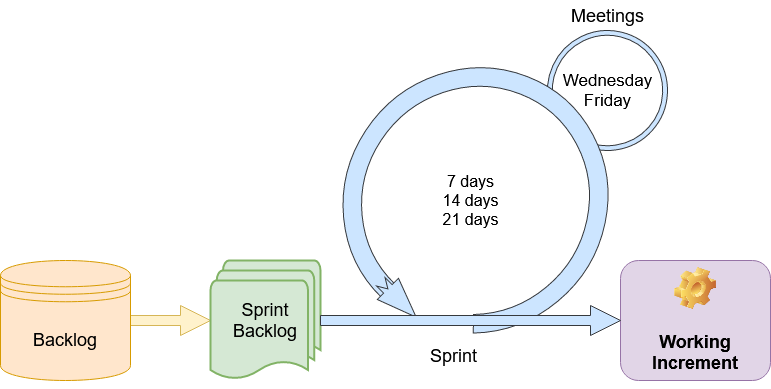
\includegraphics[width=0.85\textwidth]{pictures/diagramms/Development-model.png}
		\caption{Development Model}
		\label{developmentmodel}
	\end{figure}

	\section{Roles}
	The roles were assigned for each milestone, it was assured that each person held at least two roles throughout the project. The roles have been assigned as follows:
	\begin{itemize}
		\item Scrum master / Project leader: Organizing plenum and sprints. Push decision making.
		\item Product owner: Take care of the backlog
		\item Kanban master: Takes care of the Kanban board
		\item Foreign minister: External representation and organization of project day. The foreign minister role is excluded from the milestone role changes.
		\item Group leader: Organization of the expert groups, leading and preparing the weekly meetings.
		\item Quality assessment: check documents and code for errors.
	\end{itemize}
	
	\section{Software}
	The following applications or services have been used in the organization of the project:
	\begin{itemize}
		\item Microsoft teams: Chat interaction, wiki, protocols, presentations.
		\item Trello: Kanban board
		\item Github: Repository for the project code
		\item Jitsi: Online conference tool
		\item Discord: Online communication tool
		\item Draw.io: Online tool for creating diagrams 
	\end{itemize}  

	\section{Corona}
	Due to the outbreak of the Coronavirus and the following regulations access to the HSR was no longer possible as of 16.03.2020. Therefore the following development has been done with the gazebo simulator.
	The meetings have been carried out via \textit{Jitsi} and \textit{Discord}. An additional project computer has been provided to run the simulation.
	The project day and RoboCup have been canceled.
	
\end{document}
